\section{Massively Learning Activities} \label{section: MLA}
\begin{itemize}
    \item \textcolor{red}{We are contracted by CNMI to create an infrastructure where we can perform data analytics on PHI. This infrastructure is hosted on-prem first, hybrid later.}
    \item \textcolor{red}{Tenants (e.g. APCD, CMNI, CMA, Criminal Justice) has the data ready.}
    \item \textcolor{red}{Data is submitted from tenants to ETL (data-pipeline) to be processed then sent to SAS (on-prem servers).}
    \item \textcolor{red}{Data analytics is performed on the data using advanced algorithms in SAS programming language}. 
    \item \textcolor{red}{Project is time sensitive, deadline is requiring TASI to move onto the development stage with existing on-prem hardware as proof-of-concept ASAP}.
    \item \textcolor{red}{Initially architect the infrastructure using existing on-prem hardware to speed up deployment}
    \item \textcolor{red}{Once deployed, stable, and proof-of-concept ready, move onto the production stage by acquiring new hardware and migrating the previous (virtualized) SAS deployment to the new hardware using vMotion.}.
    \item \textcolor{red}{Configure the security relationship between the software, hardware, and tenants (Active Directory, LDAP, Security Groups, etc}.
\end{itemize}

The System Development Lifecycle (SDLC) is a project management model that defines different stages that are necessary to bring a project from conception to deployment and later maintenance. Massively Learning Activities will follow a similar variation to the SDLC project management model where each SDLC stage corresponds to a subsection in this chapter. 

\subsection{Planning Stage}
Massively Learning Activities (MLA) is divided into two phases, (1) the initial deployment of SAS on existing infrastructure and later (2) the migration of SAS onto scaled infrastructure. 

In either deployment stage, SAS Viya will be deployed in a multi-tenant environment. A multi-tenant deployment of SAS Viya allows for a single deployment to serve multiple customers\footnote{Customers are tenants (etc: CNMI, APCD, CMA, Med-Quest, UH Education) but each tenant has its own set of users and groups.}. These customers can share some physical resources while remaining logically separated. A multi-tenant deployment allows for these distinct groups to share IT resources in a secure and cost-effect manner. Multi-tenancy deploys into a \href{https://kubernetes.io/}{Kubernetes} namespace. The deployment includes a provider tenant, shared mid-tier services, application-specific database schemas, shared applications, and a designated SAS administrator for the provider tenant. Administrators with elevated Kubernetes privileges onboard one or more tenants. After tenant on-boarding, Kubernetes administrators onboard one or more Cloud Analytic Services into each new tenant, then each CAS server is uniquely configured during the on-boarding process to meet the specific tenant requirements. 

The final and completed deployment of SAS Viya will expect a total of 8 tenants:

\begin{itemize}
    \item \textbf{Tenant 1}: Commonwealth of the Northern Mariana Islands (CNMI)
    \item \textbf{Tenant 2}: All-Payer Claims Database (APCD)
    \item \textbf{Tenant 3}: Centers for Medicare \& Medicaid Services (CMA)
    \item \textbf{Tenant 4}: Med-Quest
    \item \textbf{Tenant 5}: UH Education 1
    \item \textbf{Tenant 6}: UH Education 2
    \item \textbf{Tenant 7}: UH Education 3
    \item \textbf{Tenant 8}: UH Education 4
\end{itemize}

%\textcolor{red}{\lipsum[1-1]}

MLA is a time sensitive project that requires deployment of SAS Viya in a multi-tenant environment as soon as possible. Therefore, an initial deployment of SAS Viya and SAS DMA will be conducted on existing on-premise infrastructure with only half the amount of tenants by \textcolor{red}{Q4 2023}. 

\subsubsection{Initial Deployment}
\textbf{HARDWARE}

The initial deployment of MLA will involve installing SAS on existing infrastructure\footnote{Infrastructure is used to describe existing hardware available to use on-premises at TASI/PHIDC.}. The existing infrastructure is  an available Dell PowerEdge FX2 Enclosure located in TASI's NOC. The PowerEdge FX2 Enclosure is a 2U hybrid rack-based computing platform that combines multiple blades\footnote{Blades are complete servers in a smaller form factor that have their own CPU(s), memory, storage, and networking components.} into a single enclosure to increase the efficiency and reduce the cost of rack-based systems. This multi-blade enclosure has a \textcolor{red}{XXGB} connection to a \textcolor{red}{storage pool (describe me)}.

\begin{figure}[H]
    \centering
    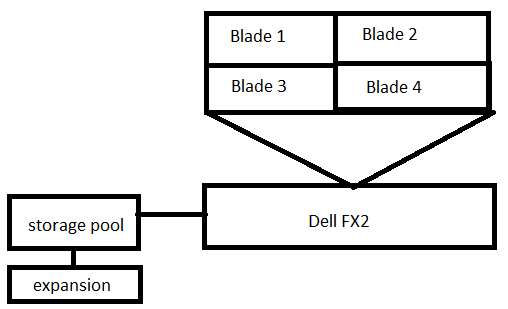
\includegraphics[scale = 0.5]{images/currentENV.png}
    \caption{TASI On-Premise Environment \textcolor{red}{(needs VISIO)} }
    \label{Current ENV}
\end{figure}

Note that each blade in the FX2 chassis is already in use by other TASI projects. Therefore, the multi-tenant SAS architecture will be logically separated based on the available resources within each blade. Each blade is uses \textbf{ESXi 6.7} as the host operating system and is equipped with \textbf{12 CPU(s)}, \textbf{256GB} of RAM, and \textcolor{red}{\textbf{XXGB}} of personal storage.

CNMI, APCD, CMA, and Med-Quest will be the initial four tenants with each tenant having a specific deployment configuration based on their respective requirements. As of \textcolor{red}{March 5, 2023}, CNMI and APDC will be configured in a 5-server environment \footnote{5 Server: (1) Primary CAS Controller, (2) Backup CAS Controller, (3) CAS Worker 1, (4) CAS Worker 2, (5) CAS Worker 3} and every other tenant will be configured in a 3-server environment\footnote{3 Server: (1) Primary CAS Controller, (2) Backup CAS Controller, (3) CAS Worker 1}. The other tenants that are yet to be added will be considered during the migration stage of MLA. 

\begin{figure}[H]
    \centering
    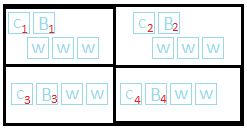
\includegraphics[scale = 1]{images/sas-initial-deployment.png}
    \caption{SAS Initial Deployment \textcolor{red}{(needs VISIO)} }
    \label{SAS Initial Deployment}
\end{figure}

\emph{Considerations:} Should the CAS Controller, CAS Backup Controller, and or CAS Worker be logically separated in the same or different hardware? 

Virtualizing the CAS Controller and Backup Controller on the same hardware can offer several benefits, such as cost savings, simplified management, and easier backup and recovery processes. However, it will be better to virtualize them on separate hardware as each tenant requires high availability and redundancy for their CAS Controllers. As for virtualizing the CAS Workers, it is recommended to virtualize them on separate hardware to reduce resource conflicts but it is not necessary. 

MLA will configure the CAS servers based on the sizing recommendations from SAS, in a highly available and redundant environment. 

\textbf{SOFTWARE}
stuff, using vmware, logically separate them, install rhel as the main OS, and then install SAS viya and DMA. make sure that the controller and backup are on different blades because that will not make sense 

\textbf{Security}
\begin{itemize}
    \item LDAP
    \item VMware Security Policies
    \item SAS Security Policies
    \item HIPPA, other Federal Laws
\end{itemize}

\textbf{}

\subsubsection{Migration Deployment}
The migration deployment of MLA will involve the migratin ghte vm's we ssetup in the intial deployment using vmware software suite VMotion. Vmotion!.

\subsection{Requirements of Analysis Stage (Sizing)}
\textcolor{red}{Refer to the sizing documents (2) and the current resources document comparison to see what we are missing.}

\subsection{Design and Prototyping Stage}

\subsection{Initial Development Stage}

\subsection{Testing Stage}

\subsection{Implementation and Integration Stage}

\subsection{Migration Stage (SDLC II)}

\subsection{Operations and Maintenance Stage}

\subsection{End-Game Implementation}
\textcolor{red}{environmental scan for the future environment}